\section{Infrastructure}\label{sec:infrastructure}

This section examines the {\em infrastructure} that people in home
networks use to access the Internet. We look at the typical composition
of devices in home networks, be they wired or wireless, and
operate either in the 2.4~GHz or the 5~GHz
wireless spectrum. Table~\ref{tab:infrastructure-results} summarizes the main
results from this section.

%\begin{itemize}
%\item Todo - CDF of fraction of times devices seen (developed v developing countries)
%\end{itemize}

\begin{figure}[t]
%\centering
%\includegraphics[width=0.9\linewidth]{figures/count_of_devices}
%\centering  \includegraphics[width=\linewidth]{figures/health/region_stat/region_stat_cdf}
\centering  \includegraphics{figures/health/region_stat/region_stat_cdf}
  \caption{Number of devices in each home network.  More than half of the homes
  have at least five devices. Each home network has seven devices on average.} 
  \label{fig:countofdevices}
\end{figure}



%unique devices median, ignore devices on 5GHz in countries where 5GHz is not allowed
\begin{figure}[t]
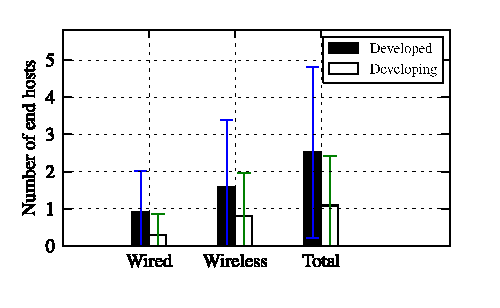
\includegraphics{figures/health/region_stat/region_stat_combined}
  \caption{Average number of devices connected to the access point at any time
  with error bars showing the standard deviation.  We see that there are more
  wireless devices in both regions. Developed has more devices overall, and
  an even greater number of wired devices.}
  \label{fig:avg_by_region}
\end{figure}


\begin{figure}[t]
  \includegraphics{figures/health/region_stat/region_stat_combined_wl}
\caption{Average number of wireless devices connected at any given time per
spectrum with error bars showing the standard deviation.  There are
significantly more devices on 2.4~GHz than on 5~GHz.}
  \label{fig:avg_spectrum_by_region}
\end{figure}


\subsection{How many devices?}\label{sec:devices}

\fp {\bf More devices in \developed{} countries.}
%TODO: might change with Joon's new plots
Figure~\ref{fig:countofdevices} shows a CDF of the number of devices
seen in each home; twenty percent of networks had at least
two unique devices, and more than half of homes had at least five
unique devices.
Figure~\ref{fig:avg_by_region} details the number of devices for
\developed{} and \developing{} countries. 
Developed countries have, on average, one more device connected to
the access point at any given time than \developing{} countries.
%This discrepancy is more pronounced in wired devices than in wireless.
%Households in \developed{} countries tend to have more devices or
%``gadgets'' in use, especially wired (it is possible that devices such as gaming consoles
%and entertainment devices, which tend to be wired, are responsible for this discrepancy).
All in all, households in countries with higher economic standards tend
to have more devices in their network, and this number is more pronounced for
wired devices. We assume this is because gaming consoles (\eg, XBox,
Playstation, Wii) or entertainment devices (\eg, Apple TV, Google TV,
Squeezebox) are more common in \developed{} countries.

\begin{table}[t!]
\begin{small}
\begin{tabular}{|p{2.6in}l|}
\hline
& \\
In \developed{} countries, 43\% of home networks have at least one
always-on wired device; only 12\% of home networks in \developing{}
countries have such as device. & \S\ref{sec:devices},
Tab.~\ref{tab:always-conn} \\ & \\ 
%
The 2.4~GHz spectrum is significantly more crowded; the median number of
devices seen on the 2.4~GHz spectrum is five, whereas on the 5~GHz band,
the median number of devices is two. & \S\ref{sec:spectrum},
Fig.~\ref{fig:cdf-devices} \\ & \\ 
%
The median number of access points seen from a home network in
\developed{} countries is about 20; in contrast, home networks in
\developing{} countries see a median of about two access points &
\S\ref{sec:spectrum}, Fig.~\ref{fig:cdf-aps} \\ & \\ 
\hline
\end{tabular}
\end{small}
\caption{Highlights of Section~\ref{sec:infrastructure} results.}
\label{tab:infrastructure-results}
\end{table}


\if 0
%%
\begin{table}[t]
\small
\begin{tabular}{ |r|r| }
  \hline
  {\bf Number of Devices} & {\bf Fraction of Homes} \\
  \hline
  at least 3 & 28/28 (100\%) \\
  6 & 23/28 (82\%) \\
  9 & 16/28 (57\%) \\
  12 & 8/28 (29\%) \\
  15 & 5/28 (28\%) \\
  18 & 2/28 (7\%) \\
  \hline
\multicolumn{2}{|r|}{Average: 9 devices} \\
  \hline
\end{tabular}
\centering\caption{Number of devices present per each
  household. \xxx{make this a CDF}}
\label{tab:countofdevices}
\end{table}
%%
\fi

\fp {\bf More ``always-connected'' devices in \developed{} countries.}
Table~\ref{tab:always-conn} shows the number of households that have at least
one wired or wireless device that never disconnects from the home gateway router
for over five weeks and its percentage against the total number of households.
The portion of households that have at least one ``always-connected'' device in
\developing{} countries is significantly lower than for \developed{} countries.
Media entertainment boxes are an example of a wired device that
never disconnects from the router, and a wireless VoIP phone is an
example of an ``always-on'' wireless device.  Some households may never
turn off their desktop or laptop.
Although we do not explore the reasons for such connectivity in depth,
we assume that households in \developing{} countries tend to power off devices
when not in use, possibly to minimize electricity 
or data usage.  Unexpected and frequent power
outages in these countries also affect device connectivity.
%%
%TODO: Table 3: Show graphs? (column 3) - parameters to be explored; maybe per 12 hour or something
\begin{table}[t]
\small
\begin{tabular}{m{0.15\columnwidth}|m{0.1\columnwidth}|m{0.26\columnwidth}|m{0.26\columnwidth}}
{\bf Group} & {\bf Total houses} & {\bf Houses with always-connected wired device} & {\bf Houses with always-connected wireless device}\\
\hline
{\developed{}} & {79} & {34 (43\%)} & {16 (20\%)}\\
{\developing{}} & {34} & {4 (12\%)} & {4 (12\%)}\\
\end{tabular}
\centering\caption{Number of households that has one or more wired or wireless device which
never disconnects from the home gateway router for over five weeks.}
\label{tab:always-conn}
\end{table}
%%



%there would
%be much less 5~GHz-capable devices than 2.4~GHz %as it is only built in the
%latest wireless devices today.

%\fp {\bf More devices used in developed countries.}
%The Figure shows that developed countries tend to have more devices (wired and
%wireless) attached in general when compared to developing countries. This can
%be caused by many reasons. 



\subsection{Wired or wireless?}

\fp {\bf More wireless than wired.}
Figure~\ref{fig:avg_spectrum_by_region} shows the average number of wired and wireless
devices attached to (and associated with) the home router 
over two
weeks, measured hourly, for \developed{} and \developing{} router groups. 
There are generally more wireless devices than wired devices.
Although this observation could reflect limitations of the router, which has only four available wired ports,
  the average number of wired ports used is
less than one in both groups; this shows that many households use wireless
even though wired connections generally
provide better throughput, latency, and stability.  This result also confirms the trend of moving away from wired
communication~\cite{www-itu} and towards primarily using wireless devices access the
Internet. For many households, wireless technology has
developed to the point where it is good enough for day-to-day Internet usage, and wired communication has little more to offer.

On the other hand, our results also suggest that wired devices are still in fairly widespread
use in some homes.  Chetty \ea stated that home users still desire wired communication
for reliability, speed, and security~\cite{Chetty:2007:SHL}.  Due
to the physical constraint of wired communication (\ie, 
cabling) devices using wired ports are likely stationary ones such as
desktop machines, network printers or media entertainment gadgets like
Apple TV. Even in homes with wired devices, our analysis suggests that a typical home gateway router
could likely suffice with only two ports. Surprisingly, only a few
households use all four Ethernet ports (9\% for both \developed{} and \developing{}
countries).
%There are few households that actually max out their wired ports
%($4$ in total) on the home gateway router.


\subsection{How much is each spectrum used?}\label{sec:spectrum}

Spectrum contention is an important problem in home wireless
networks. Many devices talking to many access points in the vicinity
causes contention and interference problems, which in turn reduces the
available bandwidth of the wireless channel. Our results confirm that
the 2.4~GHz spectrum is quite crowded, especially in \developed{}
countries, which could create bottlenecks as access link throughputs
continue to increase.  The 5~GHz spectrum, on the other hand, is less
crowded (at least for now).

\fp {\bf Wireless spectrum usage.}
Figure~\ref{fig:avg_spectrum_by_region} shows that there are more
devices active on the 2.4~GHz spectrum than on the 5~GHz spectrum at any
given time. This phenomenon may result from the fact that dual-band
devices are more expensive, and single-band devices default to the more
popular 2.4~GHz spectrum. Phones are equipped almost exclusively with
only 2.4~GHz radios.  Figure~\ref{fig:cdf-devices} shows a CDF of the
total number of {\em unique} devices seen per household. We see that the
median number of devices on the 2.4~GHz spectrum is five, while the
median number of devices on the 5~GHz spectrum is two.

We see a similar trend in the number of other access points seen on both
spectrums. The median number of other access
points is only about one device in the 5~GHz spectrum, while it is higher
for the 2.4~GHz spectrum, as expected.
Figure~\ref{fig:cdf-aps} shows a CDF
of the total number of unique access points seen per household. 
Scanning is done only in the channel the access point is configured in
(channel 11 for 2.4~GHz by default, though the user can configure it),
so this does not tell us all
the access points available, but it does tell us how likely it is
that interference occurs due to competing access points. We see that
the 2.4~GHz spectrum is more densely occupied in \developed{} countries,
and interestingly, we see
that there are two modes in both sets; either there are
very few access points in that channel or there are a lot (more than ten in \developed{}
and more than three in \developing{} countries).
%We hypothesise that this is
%an indication of users living in apartments versus those in homes.
%Figure~\ref{fig:avg_spectrum_by_region} shows that there are more devices
%active on the 2.4~GHz spectrum than 5~GHz at any given time. This seems mostly
%due to the fact that dual band devices are more expensive, and single-band
%devices default to the more popular 2.4~GHz spectrum. Phones are equipped
%almost exclusively with only 2.4~GHz radios.  Figures~\ref{fig:cdf-2-devices}
%and~\ref{fig:cdf-5-devices} show the CDF of the total number of unique devices
%seen per household.
%
%Figures~\ref{fig:cdf-2-aps} and~\ref{fig:cdf-5-aps} show the CDF
%of the total number of unique access points seen per household. The 
%scanning is done only in the channel the access point is configured in
%(channel 11 for 2.4~GHz and 36 for 5~GHz), so this does not tell us all
%the access points available, but it does tell us how likely it is 
%that interference occurs due to competing access points. We see that
%the 2.4~GHz spectrum is more densely occupied, and interestingly, we see
%that there are two modes in the developed countries; either there are
%very few access points in that channel or there are a lot ($>$ 10).
%Also, as expected, the spectrum is more polluted in the developed countries.
  
%About 10\% of the devices in our data set are dual-band capable.
%Figure~\ref{fig:cdf-frac-5} shows the fraction of time such devices use the
%5~GHz spectrum. We expected to see that devices almost exclusively use either
%one or the other (based on initial configuration), but surprisingly there seems
%to be no real pattern; devices are almost equally likely to stick to one
%spectrum as they are to hop between different spectrums.



%fig 7: TODO any other way to show this figure
\begin{figure}[t]
  \begin{minipage}{\linewidth}
  \includegraphics{figures/cdf_clients_all}
  \caption{Number of unique devices seen on the two wireless
    spectrums. The median is about five devices on 2.4~GHz and two
    devices on 5~GHz.} 
  \label{fig:cdf-devices}
%  \subfloat[Median number of devices seen on 2.4~GHz spectrum is 5]{
%  \includegraphics[width=0.98\linewidth]{figures/cdf_clients_wlan0}
%  \label{fig:cdf-2-devices}}\\
%  \subfloat[Median number of devices seen on 5~GHz spectrum is 2 (among homes which see devices in the 5 spectrum)]{
%  \includegraphics[width=0.98\linewidth]{figures/cdf_clients_wlan1}
%  \label{fig:cdf-5-devices}}
%  \caption{Number of devices seen on the two spectrums}
%  \label{fig:cdf-devices}
  \end{minipage}
\end{figure}

%fig 6
\begin{figure}[t]
  \begin{minipage}{\linewidth}
  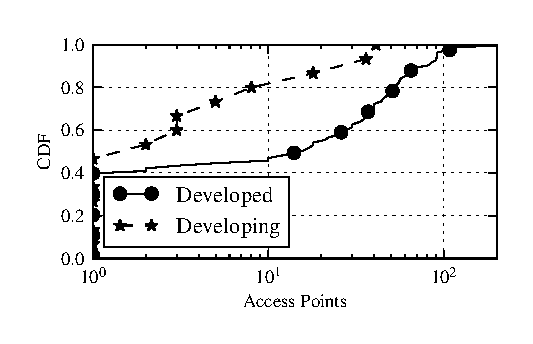
\includegraphics{figures/cdf_aps_all}
  \caption{Number of access points seen on the 2.4~GHz spectrum in \developed{} and \developing{} countries. There are many more access points visible in \developed{}, where we see modal behavior with either very few or a lot of neighboring access points.}
  \label{fig:cdf-aps}
%  \subfloat[Median number of APs seen on 2.4~GHz spectrum is about 10 in developed countries]{
%  \includegraphics[width=0.98\linewidth]{figures/cdf_aps_wlan0_rc}
%  \label{fig:cdf-2-aps-rc}}\\
%  \subfloat[Median number of APs seen on 2.4~GHz spectrum is 2 in developing countries]{
%  \includegraphics[width=0.98\linewidth]{figures/cdf_aps_wlan0_nsrc}
%  \label{fig:cdf-5-aps-nsrc}}
%  \caption{There is a clear bimodal pattern in the number of APs seen}
%  \label{fig:cdf-2-aps}
  \end{minipage}
\end{figure}




%TODO this paragraph doesn't seem important for IMC

%% \paragraph{How many devices are capable of dual band?}
%% About 10\% of the devices in our data set are dual-band capable.
%% Figure~\ref{fig:cdf-frac-5} shows the fraction of time such devices use the
%% 5~GHz spectrum. We expected to see that devices almost exclusively use either
%% one or the other (based on initial configuration), but surprisingly there seems
%% to be no real pattern; devices are almost equally likely to stick to one
%% spectrum as they are to hop between different spectrums.
%% %TODO: implication may change with new plots

%% %TODO: is this valid? need to redo plot
%% \begin{figure}[t]
%% \includegraphics[width=0.98\linewidth]{figures/cdf_frac_5_usage}
%% \caption{Among dual-band devices, there is no discernible preference for either
%% 2.4 or 5~GHz}\label{fig:cdf-frac-5}
%% \end{figure}

%\subsection{Usage patterns of wireless devices}
%Figure~\ref{fig:diurnal-all} shows the usage patterns of all wireless devices
%across a day, broken down into weekday (Monday-Friday) and weekend. We see that
%there is a clear diurnal pattern in the number of unique devices seen at
%various times of the day during the weekday. Usage peaks during the evenings,
%and troughs during the afternoons. The wireless devices could be either laptops
%or cellular devices. We see that the number of devices dips only slightly at
%night (compared to the dip during the day), so it's most likely to be cellular
%devices, as laptops are more likely to be switched off at night. On weekends,
%we see no discernible diurnal patterns.

%\begin{figure}
%  \begin{minipage}{\linewidth}
%  \subfloat[Median number of APs seen on 5~GHz spectrum is about 2 in developed countries]{
%  \includegraphics[width=0.98\linewidth]{figures/cdf_aps_wlan1_rc}
%  \label{fig:cdf-5-aps-rc}}\\
%  \subfloat[Median number of APs seen on 5~GHz spectrum is 1 in developing countries]{
%  \includegraphics[width=0.98\linewidth]{figures/cdf_aps_wlan1_nsrc}
%  \label{fig:cdf-5-aps-nsrc}}
%  \caption{The number of APs seen in 5~GHz is much lower than on 2.4~GHz}
%  \label{fig:cdf-5-aps}
%  \end{minipage}
%\end{figure}
%
%
%
%\begin{figure}[t]
%\includegraphics[width=0.98\linewidth]{figures/cdf_frac_5_usage}
%\caption{Among dual-band devices, there is no clear preference for 2.4 or 5}\label{fig:cdf-frac-5}
%\end{figure}

\subsection{Which device vendors are most common?}\label{sec:deviceVendors}

For the 25 homes in the United States in the Traffic data set, we observed the
frequency of various types of devices connected to the home network. When
collecting the Traffic data set, we obfuscate the bottom 24 bits of the MAC
addresses of all devices seen by the gateway. The first 24 bits allow us to look
up the manufacturer, and though this does not always tell us if the device is a
phone, tablet, or laptop, it still provides us enough information to distinguish
network gateways from smart devices and wireless cards.

\begin{figure}[t!]
%filtered to devices atleast > 100 KB data in 15 days -- misses the printers
\includegraphics[width=\linewidth]{figures/devices_seen_filtered}	
%\includegraphics[width=\linewidth]{figures/devices_seen_v2}			%unfiltered
\caption{The number of devices seen in the Devices data set across
  all homes in the Traffic data set (25 homes in the United States).
  We only considered devices which transferred at least 100 KB. }
 \label{fig:manufacturer}
\end{figure}



Based on passive monitoring of 25 homes, Figure~\ref{fig:manufacturer} plots the
device types seen in the Traffic data set. We have removed all
references to Netgear originating from our BISmark routers. The most common device was manufactured by Apple, followed by Intel.  Other Samsung and smart phones
were also reasonably common.\footnote{ The {\em
  Printer} manufacturer was an Epson. {\em Hardware} includes Giga-Byte
and Microchip.  {\em VoIP} is a UniData device.  {\em Internet TV}
includes Roku, TiVo, and ASRock home theatres.  {\em Wireless Card}
includes AzureWave and GainSpan. {\em Gaming} includes Nintendo and
Mitsumi (which manufactures controllers for Playstations, Xbox, and
Wii).  Microsoft (possibly Xbox) is shown separately. Gateway includes
TP-Link, Realtek, Liteon, D-Link, Cisco-Linksys, Belkin, and Askey. {\em
  Smart Phones} includes HTC, LG, Motorola, Nokia, and a confirmed
Samsung Galaxy S II (Murata Inc.).  Other Samsung devices, including
phones and tablets, are shown separately.  {\em Original Device
  Manufacturers (ODMs)} include Compal, Hon Hai Precision, Quanta,
Universal Global Systems, Winstron Infocomm. Misc. includes Polycom (a
telecom product manufacturer), Prolifix (which makes Internet-enabled
thermostats), and Pegatron (which manufactures a variety of products
including notebooks, laptops to gateways).}  We recently started
gathering Traffic data in several \developing{} countries, so we will soon
be able to compare the distribution of device manufacturers in \developed{}
and \developing{} countries.
